\section{Experiments}
\label{sec:experiments}

\subsection{Experimental Setup}
\label{sec:setup}

\paragraph{Benchmark.}
We evaluate on EndoBench~\cite{liu2025endobench}, which contains $6{,}832$
clinically reviewed multiple-choice VQA pairs across four endoscopic scenarios,
four clinical categories, and 12 tasks. Controller-training questions are
independently constructed from Chinese medical books without using EndoBench
question--answer pairs.

\paragraph{Models and retrieval environment.}
The frozen generator is Qwen3-VL-8B-Instruct and the trainable controller is
Qwen3.5-4B. BGE-M3 serves as the text retriever and the Qwen3-VL image encoder
as the image retriever. The deployed index holds $230{,}004$ knowledge units
built from $431$ Chinese endoscopy and gastroenterology books and atlases:
$163{,}713$ text units and $66{,}291$ image--text pairs. Each channel retrieves
its top 20 neighbors from a Milvus index with \texttt{nprobe}=64, and the top
six candidates per channel form a 12-item controller pool. The examination
type routes retrieval to a compatible \texttt{body\_site\_main} partition; this
is the endoscopy-type field that the benchmark supplies with every question, it
is independent of the gold option, task label, and evaluation category, and
surgical endoscopy carries no single anatomical site and therefore searches the
full index. An optional frozen Mengzi-based density and visual-dependence
module predicts query-specific channel weights for front-end ablations; the
reported 42.84\% configuration uses equal text/image quotas and does not enable
it. Every rewrite otherwise traverses the same frozen retrieval path. The
generator predicts by normalizing next-token logits over valid answer options.

\paragraph{Training.}
SFT uses $3{,}327$ teacher trajectories to learn the structured action schema,
candidate-level selection, sufficiency decisions, and query rewriting. RFT uses
$2{,}069$ generator-utility-filtered policy trajectories balanced across
rewrite-win, selection, and trivial states. GRPO uses $1{,}672$
retrieval-need-aware states with eight actions per group. We use a learning rate
of $3\times10^{-6}$, KL coefficient $0.02$, temperature $1.4$, and top-$p$
$0.95$. We select checkpoint u50 for its balance of utility and structured
output reliability.

\paragraph{Compared configurations.}
A round is one controller decision. All configurations share the same frozen
retrievers, index, and generator, and the same controller checkpoint wherever a
controller is used. \emph{One-shot RAG} supplies all 12 initial candidates to
the generator. The \emph{single-round agent} makes one decision: \textsc{Accept}
uses its retained subset, whereas \textsc{Rewrite} retrieves once and supplies
the top five redirected candidates. The \emph{memoryless iterative agent}
(R3-NM) allows up to three decisions but keeps no cross-round state: it stops on
\textsc{Accept} and discards earlier candidates and traces after rewriting, so
every decision sees only the current pool; empty or failed decisions use a
deterministic top-five fallback.

\emph{AgenticRL Full} adds trajectory-aware memory. Since retained evidence is
reusable only if a later round exists, memory is deployed inside a three-step
budget and \textsc{Accept} does not terminate: an accepted non-empty
\textsc{Keep} set replaces $M^+$ and the next step re-evaluates it without
retrieval, whereas \textsc{Rewrite} reruns the frozen chain and appends the
refuted query and its rejected candidates to the controller-only $M^-$. An
initial \textsc{Rewrite} deterministically initializes $M^+$ with the top three
current candidates, parse failures skip state updates, and questions with no
retained evidence reuse the single-round prediction. Memory and this wrapper are
co-designed rather than independent: the wrapper holds no information of its
own, and we isolate the state by a protocol-matched ablation that switches only
$M^+$/$M^-$ and by separating questions on which memory becomes active.

\paragraph{Metrics.}
We report accuracy, absolute improvement, mean retrieval calls, and paired
outcome transitions. Correction rate is the fraction of single-round errors
made correct; regression rate is the fraction of single-round correct answers
made wrong. Confidence intervals use $B=10{,}000$ paired bootstrap resamples,
and paired accuracy changes use two-sided exact McNemar tests.

\subsection{Main Results}
\label{sec:main-results}

\begin{table}[t]
  \centering
  \small
  \begin{tabular}{lcrrr}
    \toprule
    Configuration & State & Acc. & $\Delta$ vs.\ SR & Calls \\
    \midrule
    \multicolumn{5}{l}{\emph{Accuracies reported by EndoBench (no retrieval)}}\\
    Gemini-2.5-Pro & -- & 49.53 & -- & -- \\
    GPT-4o & -- & 41.69 & -- & -- \\
    MedDr-80B & -- & 39.96 & -- & -- \\
    HuatuoGPT-Vision-34B & -- & 39.58 & -- & -- \\
    \midrule
    \multicolumn{5}{l}{\emph{Shared frozen stack (ours)}}\\
    Qwen3-VL-8B closed-book & -- & 40.59 & +0.47 & 0 \\
    One-shot RAG & -- & 38.85 & -1.27 & 1.00 \\
    Single-round agent (SR) & No & 40.12 & \phantom{+}0.00 & 1.53 \\
    Iterative agent (R3-NM) & No & 39.56 & -0.56 & 1.87 \\
    AgenticRL Full & Yes & \textbf{42.84} & \textbf{+2.72} & 2.39 \\
    \bottomrule
  \end{tabular}
  \caption{Results on all $6{,}832$ EndoBench questions; the upper block
  reproduces accuracies reported by~\citet{liu2025endobench}. ``State''
  indicates whether cross-round memory ($M^+$/$M^-$) is maintained, and Calls is
  the mean number of retrieval calls per question. Within the shared frozen
  stack, iteration without memory does not improve over a single round, whereas
  memory-aware control adds $3.28$ points over it (exact McNemar
  $p=2.1\times10^{-13}$). With a 4B controller over a frozen 8B generator,
  AgenticRL also surpasses the GPT-4o accuracy reported for this benchmark.}
  \label{tab:main}
\end{table}

\paragraph{Iteration alone does not help; evidence-preserving iteration does.}
One-shot RAG reaches 38.85\%, 1.74 points below the 40.59\% closed-book
generator: unfiltered evidence hurts. One controller decision recovers 1.27
points to 40.12\%. Allowing up to three decisions \emph{without} cross-round
state does not improve this but slightly degrades it: the memoryless iterative
agent obtains 39.56\%, 0.56 points below the single-round agent, because each
new query is formulated from the current pool alone, so earlier useful
candidates are lost and refuted directions can be revisited. Carrying
trajectory-aware state across rounds turns iteration into a gain: with the same
controller and stack, AgenticRL Full reaches 42.84\%, $+3.28$ points over
memoryless iterative control (578 questions become correct against 354 that
become wrong; exact McNemar $p=2.1\times10^{-13}$, paired bootstrap 95\% CI
$[+2.40,+4.14]$) and $+2.72$ points over single-round control
($p=1.2\times10^{-12}$, CI $[+1.98,+3.47]$). It also improves the closed-book
generator by 2.25 points ($p=6.6\times10^{-4}$) and one-shot RAG by 4.00 points
($p=5.3\times10^{-17}$). As stated above, the two iterative protocols differ in
execution because $M^+$ cannot be exploited without a subsequent round, so this
contrast measures the complete evidence-preserving strategy; the next two
analyses quantify how much of it the state itself carries.

\paragraph{The gain is concentrated where memory is active.}
Memory is not a nominal component: across the $16{,}299$ executed rounds, $M^+$
is non-empty in $9{,}380$ rounds with a mean of $3.66$ retained items, and
$M^-$ carries at least one refuted query in $6{,}166$ rounds. We call a question
\emph{memory-active} if at least one round presents a non-empty $M^+$ or $M^-$
to the controller, which holds for $6{,}811$ of $6{,}832$ questions. This set
carries the entire benchmark-level gain: 435 of the 436 corrected questions, an
improvement of $3.26$ points over memoryless iterative control
($p=3.3\times10^{-13}$, CI $[+2.39,+4.16]$) and $2.73$ points over single-round
control. On the remaining 21 questions, where degenerate parses leave both
states empty and the controller therefore behaves memorylessly, accuracy is
unchanged (11 correct in both systems); this residual set is too small for a
powered test and is reported only as a consistency check.

\paragraph{Comparison with reported EndoBench systems.}
The upper block of Table~\ref{tab:main} lists accuracies reported by
EndoBench. With a frozen 8B generator and a 4B controller, AgenticRL reaches
42.84\% and exceeds GPT-4o (41.69\%) by 1.15 points, as well as the
medical-specialist MedDr-80B (39.96\%) and HuatuoGPT-Vision-34B (39.58\%), that
is, answering models four to ten times larger; Gemini-2.5-Pro (49.53\%), the
strongest reported system, remains ahead. Those systems answer directly whereas
AgenticRL consults an external index, so this comparison is secondary and
contextual rather than architecture-matched; its point is that state-carrying
retrieval control reaches this accuracy band more cheaply than scaling the
answering model. We use the shared-stack rows as the primary evidence.

\paragraph{Correction of initial errors.}

\begin{figure*}[t]
  \centering
\IfFileExists{figures/fig3_transition_final.pdf}{
  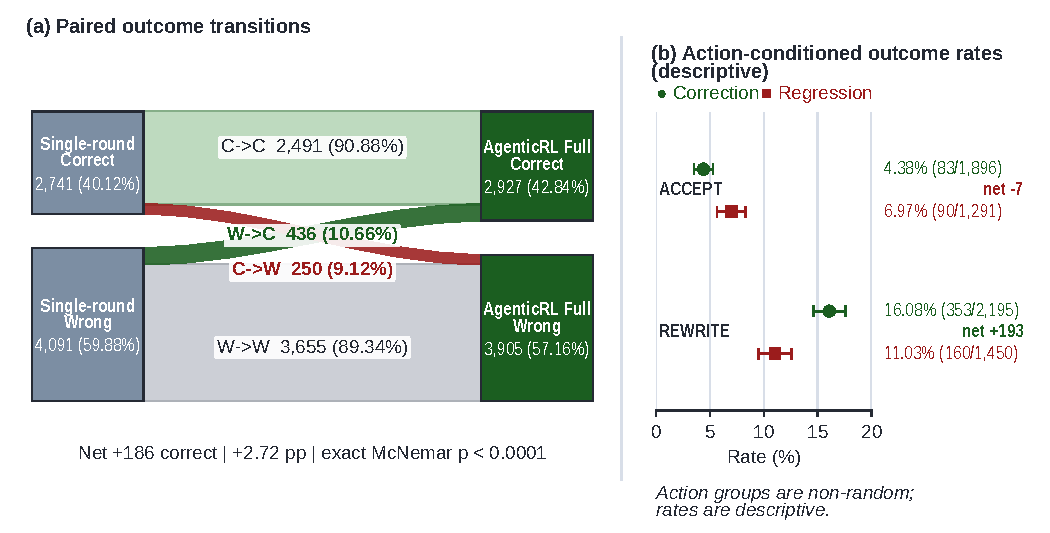
\includegraphics[width=0.92\textwidth]{figures/fig3_transition_final.pdf}
}{
  \fbox{\parbox[c][5.2cm][c]{0.94\textwidth}{\centering
  Placeholder: paired transitions and correction rates}}
}
\caption{Prediction transitions from the single-round agent to AgenticRL Full.
Panel (a) reports paired per-item outcomes under memory-aware control.
Panel (b) reports correction and regression rates stratified by the initial
controller action; this comparison is descriptive because actions are not
randomly assigned. Error bars denote stratified-bootstrap 95\% confidence
intervals with $B=10{,}000$.}
\label{fig:transitions}
\end{figure*}

The single-round agent answers 4,091 questions incorrectly. Memory-aware control
corrects 436 of them, a 10.66\% correction rate, while 250 of its 2,741 correct
predictions become incorrect, a 9.12\% regression rate; the net increase of 186
questions matches the 2.72-point gain and is significant by an exact McNemar
test ($p<0.0001$). Figure~\ref{fig:transitions} shows the complete transitions
and their stratification by the initial controller action. Of the 436
corrections, 353 were initially assigned \textsc{Rewrite} and 83
\textsc{Accept}, with correction rates of 16.08\% and 4.38\% and
non-overlapping confidence intervals, and a net gain of $+193$ questions in the
\textsc{Rewrite} group against $-7$ in the \textsc{Accept} group. Redirected
retrieval, exactly the branch that writes $M^-$ and later reuses $M^+$, is thus
where the improvement originates. This split is descriptive rather than causal
because the controller assigns actions non-randomly.

\subsection{Isolating Cross-Round State}
\label{sec:ablations}

\begin{table}[t]
  \centering
  \small
  \begin{tabular}{lcrr}
    \toprule
    Fixed-budget configuration & $M^+$/$M^-$ & Acc. & $\Delta$ \\
    \midrule
    Single-round & Off/Off & 40.22 & Reference \\
    Wrapper only & Off/Off & 41.32 & \phantom{*}+1.10 \\
    Wrapper + cross-round state & On/On & \textbf{42.61} & \textbf{+2.40*} \\
    \bottomrule
  \end{tabular}
  \caption{Protocol-matched ablation on the same stratified $1{,}002$-question
  subset; the last two rows are identical except for $M^+$/$M^-$. Only the
  memory-equipped configuration significantly improves over single-round control
  (*exact $p=0.028$, 95\% CI $[+0.30,+4.49]$); the wrapper alone does not
  ($p=0.359$). Cross-round state contributes $+1.30$ of the $+2.40$-point total,
  i.e.\ 54\% (CI $[-1.20,+3.79]$, $p=0.344$ at this subset size).}
  \label{tab:ablations}
\end{table}

Table~\ref{tab:ablations} switches only $M^+$/$M^-$ while holding the budget,
the \textsc{Accept} semantics, the top-3 initialization, the parse policy, the
fallback rule, and the generation context capacity fixed, on a stratified
$1{,}002$-question subset fixed before these runs. Under the identical
fixed-budget protocol, the wrapper without cross-round state reaches 41.32\%
from a 40.22\% single-round reference, which is not significant ($+1.10$, 95\%
CI $[-1.00,+3.19]$, $p=0.359$). Enabling $M^+$ and $M^-$ raises accuracy to
42.61\%, the only configuration that significantly improves over single-round
control ($+2.40$, CI $[+0.30,+4.49]$, exact $p=0.028$). Cross-round state
therefore contributes $+1.30$ points, the majority (54\%) of the matched
improvement, in the same direction and of comparable magnitude to the
$+3.28$-point full-benchmark contrast. Its isolated increment is not
individually significant at $n=1{,}002$ (CI $[-1.20,+3.79]$, $p=0.344$), since
an effect of this size is underpowered at that sample size, which is why the
memory contrast is also evaluated on all $6{,}832$ questions, where it is
significant. Because $M^+$ pays off only when a further round can reuse it, the
strongest evidence supports the complete fixed-budget, evidence-preserving
strategy: cross-round state is a property of budgeted execution rather than a
protocol-independent module that transfers to protocols terminating at the first
\textsc{Accept}.

\paragraph{Efficiency and reliability.}
The memoryless iterative agent averages 1.87 retrieval calls, enters multiple
rounds on 53.1\% of questions, and fails to parse on 3.59\%. The single-round
agent averages 1.53 calls because 53.35\% of questions execute an additional
rewrite retrieval. AgenticRL Full uses 2.39 calls with a 3.94\% parse-failure
rate and a 12.3\% fallback rate, since its wrapper evaluates every question for
multiple steps. The matched subset shows that memory also makes budgeted
execution cheaper and more reliable: with identical rules, the wrapper-only
configuration needs 2.63 calls, fails to parse on 5.49\%, and ends 27.9\% of
questions with no usable evidence, whereas the memory-equipped configuration
uses 2.40 calls, fails to parse on 3.79\%, and falls back on 11.18\%. Retaining
evidence across rounds thus removes more than half of the empty-evidence
outcomes while spending fewer retrieval calls, although iterative control
remains more expensive than a single round.

\subsection{Analysis}
\label{sec:analysis}

\paragraph{Clinical categories, scenarios, and tasks.}

\begin{figure*}[t]
  \centering
\IfFileExists{figures/fig4_clinical_breakdown_final.pdf}{
  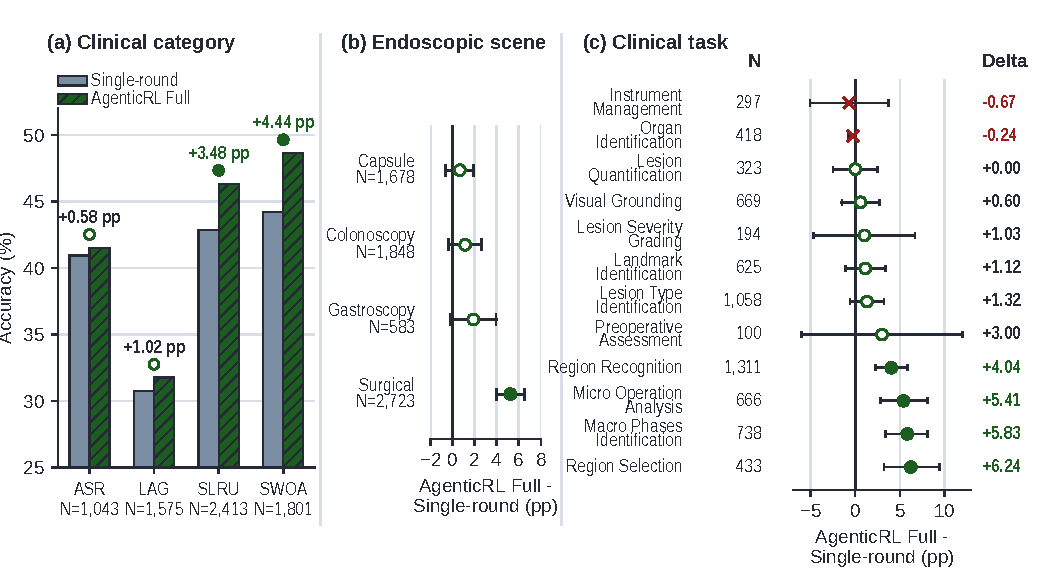
\includegraphics[width=0.90\textwidth]{figures/fig4_clinical_breakdown_final.pdf}
}{
  \fbox{\parbox[c][4.0cm][c]{0.96\textwidth}{\centering
  Pending final per-item aggregation: category accuracy, scene gains,
  and task-level gains}}
}
\caption{Clinical breakdown by category, endoscopic scenario, and task.
Panel (a) compares the single-round agent and AgenticRL Full. Panels (b) and
(c) report their paired accuracy difference in percentage points with paired
bootstrap 95\% confidence intervals ($B=10{,}000$). All groups, including
negative changes, are retained.}
\label{fig:clinical-breakdown}
\end{figure*}

The largest category-level gains occur in surgical workflow and operation
analysis (+4.44 points, $p=2.10\times10^{-7}$) and spatial localization and
region understanding (+3.48, $p=1.04\times10^{-7}$). At the scene level,
surgical endoscopy improves by 5.25 points ($p=5.97\times10^{-16}$), whereas
the other three scenes show smaller, non-significant changes. Task-level gains
are significant for region selection (+6.24), macro-phase identification
(+5.83), micro-operation analysis (+5.41), and region recognition (+4.04).
Instrument management (-0.67), organ identification (-0.24), and lesion
quantification (0.00) do not improve. The overall gain thus localizes to
spatial and procedural reasoning, where several retrieval attempts must be
accumulated and compared, rather than to tasks whose answer is already settled
by the first pool.
